\begin{frame}[fragile]{Merging cover trees}

Merging cover trees gives us a parallel tree construction algorithm

\vspace{0.15in}

Sometimes, merging cover trees is \textbf{easy}:

\begin{center}
\begin{tikzpicture}
    [ draw
    , every node/.style={minimum size=10mm,fill=white}
    , level/.style={sibling distance = 23mm/#1, level distance=12mm}
    %,    level distance = 1.5cm}
    , sibling distance=8mm
    ]
\draw (-2.3,0) -- (8.6,0)[dotted];
\draw (-2.3,-12mm) -- (8.6,-12mm)[dotted];
\draw (-2.3,-24mm) -- (8.6,-24mm)[dotted];
\node[shape=circle,draw] at (0,0) {10}
    child { node[circle,draw] {8}
        child { node[circle,draw] {7}  }
        child { node[circle,draw] {9} }
        }
    child [color=white] {}
    %child { node[circle,draw] {12}
        %child { node[circle,draw] {9}  }
        %child { node[circle,draw] {13} }
        %}
    ;
\node[shape=circle,draw,fill=lightgreen] at (5,-12mm) {12}
    %child { node[circle,draw] {8}
        %child { node[circle,draw] {7}  }
        %child { node[circle,draw,fill=lightgreen,line width=1pt] {9} }
        %}
    %child { node[circle,draw] {12}
        child { node[circle,draw] {11}  }
        child { node[circle,draw] {13} }
        %}
    ;
\node[fill=none] at (8,3mm) {level 3};
\node[fill=none] at (8,-9mm) {level 2};
\node[fill=none] at (8,-21mm) {level 1};
\end{tikzpicture}
\end{center}

\vspace{0.1in}
No runtime bound on the merge operation, but it is fast in practice

%\vspace{0.1in}
%But, if the runtime is $o(n)$, then we get an algorithm for tree construction that takes time $O(n)$
\end{frame}

%%%%%%%%%%%%%%%%%%%%%%%%%%%%%%%%%%%%%%%%%%%%%%%%%%%%%%%%%%%%%%%%%%%%%%%%%%%%%%%%

\begin{frame}[fragile]{Merging cover trees}

Merging cover trees gives us a parallel tree construction algorithm

\vspace{0.15in}

Sometimes, merging cover trees is \textbf{hard}:

\begin{center}
\begin{tikzpicture}
    [ draw
    , every node/.style={minimum size=10mm,fill=white}
    , level/.style={sibling distance = 23mm/#1, level distance=12mm}
    %,    level distance = 1.5cm}
    , sibling distance=8mm
    ]
\draw (-2.3,0) -- (8.6,0)[dotted];
\draw (-2.3,-12mm) -- (8.6,-12mm)[dotted];
\draw (-2.3,-24mm) -- (8.6,-24mm)[dotted];
\node[shape=circle,draw] at (0,0) {10}
    child { node[circle,draw] {8}
        child { node[circle,draw] {7}  }
        child { node[circle,draw] {9} }
        }
    child [color=white] {}
    %child { node[circle,draw] {12}
        %child { node[circle,draw] {9}  }
        %child { node[circle,draw] {13} }
        %}
    ;
\node[shape=circle,draw,fill=lightred] at (5,-12mm) {11.5}
    %child { node[circle,draw] {8}
        %child { node[circle,draw] {7}  }
        %child { node[circle,draw,fill=lightgreen,line width=1pt] {9} }
        %}
    %child { node[circle,draw] {12}
        child { node[circle,draw] {11}  }
        child { node[circle,draw] {13} }
        %}
    ;
\node[fill=none] at (8,3mm) {level 3};
\node[fill=none] at (8,-9mm) {level 2};
\node[fill=none] at (8,-21mm) {level 1};
\end{tikzpicture}
\end{center}

\vspace{0.1in}
No runtime bound on the merge operation, but it is fast in practice

%\vspace{0.1in}
%But, if the runtime is $o(n)$, then we get an algorithm for tree construction that takes time $O(n)$
\end{frame}

%%%%%%%%%%%%%%%%%%%%%%%%%%%%%%%%%%%%%%%%%%%%%%%%%%%%%%%%%%%%%%%%%%%%%%%%%%%%%%%%

\begin{frame}[fragile]{The effect of parallel tree \emph{construction} on small datasets}
\begin{center}
\graphicspath{{slides/paperimg/}}
% GNUPLOT: LaTeX picture with Postscript
\begingroup
  \makeatletter
  \providecommand\color[2][]{%
    \GenericError{(gnuplot) \space\space\space\@spaces}{%
      Package color not loaded in conjunction with
      terminal option `colourtext'%
    }{See the gnuplot documentation for explanation.%
    }{Either use 'blacktext' in gnuplot or load the package
      color.sty in LaTeX.}%
    \renewcommand\color[2][]{}%
  }%
  \providecommand\includegraphics[2][]{%
    \GenericError{(gnuplot) \space\space\space\@spaces}{%
      Package graphicx or graphics not loaded%
    }{See the gnuplot documentation for explanation.%
    }{The gnuplot epslatex terminal needs graphicx.sty or graphics.sty.}%
    \renewcommand\includegraphics[2][]{}%
  }%
  \providecommand\rotatebox[2]{#2}%
  \@ifundefined{ifGPcolor}{%
    \newif\ifGPcolor
    \GPcolortrue
  }{}%
  \@ifundefined{ifGPblacktext}{%
    \newif\ifGPblacktext
    \GPblacktextfalse
  }{}%
  % define a \g@addto@macro without @ in the name:
  \let\gplgaddtomacro\g@addto@macro
  % define empty templates for all commands taking text:
  \gdef\gplbacktext{}%
  \gdef\gplfronttext{}%
  \makeatother
  \ifGPblacktext
    % no textcolor at all
    \def\colorrgb#1{}%
    \def\colorgray#1{}%
  \else
    % gray or color?
    \ifGPcolor
      \def\colorrgb#1{\color[rgb]{#1}}%
      \def\colorgray#1{\color[gray]{#1}}%
      \expandafter\def\csname LTw\endcsname{\color{white}}%
      \expandafter\def\csname LTb\endcsname{\color{black}}%
      \expandafter\def\csname LTa\endcsname{\color{black}}%
      \expandafter\def\csname LT0\endcsname{\color[rgb]{1,0,0}}%
      \expandafter\def\csname LT1\endcsname{\color[rgb]{0,1,0}}%
      \expandafter\def\csname LT2\endcsname{\color[rgb]{0,0,1}}%
      \expandafter\def\csname LT3\endcsname{\color[rgb]{1,0,1}}%
      \expandafter\def\csname LT4\endcsname{\color[rgb]{0,1,1}}%
      \expandafter\def\csname LT5\endcsname{\color[rgb]{1,1,0}}%
      \expandafter\def\csname LT6\endcsname{\color[rgb]{0,0,0}}%
      \expandafter\def\csname LT7\endcsname{\color[rgb]{1,0.3,0}}%
      \expandafter\def\csname LT8\endcsname{\color[rgb]{0.5,0.5,0.5}}%
    \else
      % gray
      \def\colorrgb#1{\color{black}}%
      \def\colorgray#1{\color[gray]{#1}}%
      \expandafter\def\csname LTw\endcsname{\color{white}}%
      \expandafter\def\csname LTb\endcsname{\color{black}}%
      \expandafter\def\csname LTa\endcsname{\color{black}}%
      \expandafter\def\csname LT0\endcsname{\color{black}}%
      \expandafter\def\csname LT1\endcsname{\color{black}}%
      \expandafter\def\csname LT2\endcsname{\color{black}}%
      \expandafter\def\csname LT3\endcsname{\color{black}}%
      \expandafter\def\csname LT4\endcsname{\color{black}}%
      \expandafter\def\csname LT5\endcsname{\color{black}}%
      \expandafter\def\csname LT6\endcsname{\color{black}}%
      \expandafter\def\csname LT7\endcsname{\color{black}}%
      \expandafter\def\csname LT8\endcsname{\color{black}}%
    \fi
  \fi
  \setlength{\unitlength}{0.0500bp}%
  \begin{picture}(5040.00,3772.00)%
    \gplgaddtomacro\gplbacktext{%
      \csname LTb\endcsname%
      \put(814,1129){\makebox(0,0)[r]{\strut{}$2^{-4}$}}%
      \csname LTb\endcsname%
      \put(814,1526){\makebox(0,0)[r]{\strut{}$2^{-3}$}}%
      \csname LTb\endcsname%
      \put(814,1922){\makebox(0,0)[r]{\strut{}$2^{-2}$}}%
      \csname LTb\endcsname%
      \put(814,2318){\makebox(0,0)[r]{\strut{}$2^{-1}$}}%
      \csname LTb\endcsname%
      \put(814,2714){\makebox(0,0)[r]{\strut{}$2^{+0}$}}%
      \csname LTb\endcsname%
      \put(814,3111){\makebox(0,0)[r]{\strut{}$2^{+1}$}}%
      \put(1539,601){\rotatebox{-45}{\makebox(0,0)[l]{\strut{}yearpredict}}}%
      \put(1539,381){\rotatebox{-45}{\makebox(0,0)[l]{\strut{}(77sec)}}}%
      \put(2242,601){\rotatebox{-45}{\makebox(0,0)[l]{\strut{}twitter}}}%
      \put(2242,381){\rotatebox{-45}{\makebox(0,0)[l]{\strut{}(107sec)}}}%
      \put(2945,601){\rotatebox{-45}{\makebox(0,0)[l]{\strut{}tinyImages}}}%
      \put(2945,381){\rotatebox{-45}{\makebox(0,0)[l]{\strut{}(65sec)}}}%
      \put(3648,601){\rotatebox{-45}{\makebox(0,0)[l]{\strut{}mnist}}}%
      \put(3648,381){\rotatebox{-45}{\makebox(0,0)[l]{\strut{}(12sec)}}}%
      \put(176,2120){\rotatebox{-270}{\makebox(0,0){\strut{}normalized tree \emph{construction} time}}}%
      \put(1464,2814){\makebox(0,0)[l]{\strut{}\tiny 1}}%
      \put(1570,2619){\makebox(0,0)[l]{\strut{}\tiny 2}}%
      \put(1667,2175){\makebox(0,0)[l]{\strut{}\tiny 4}}%
      \put(1763,1967){\makebox(0,0)[l]{\strut{}\tiny 8}}%
      \put(1860,1856){\makebox(0,0)[l]{\strut{}\tiny 16}}%
      \put(1473,3230){\makebox(0,0)[l]{\strut{}number of processors}}%
    }%
    \gplgaddtomacro\gplfronttext{%
    }%
    \gplbacktext
    \put(0,0){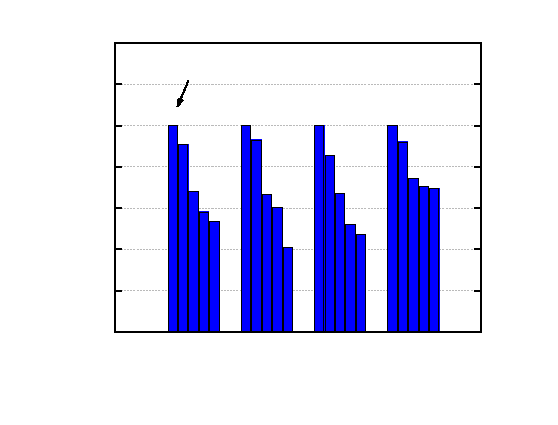
\includegraphics{parallel-ancestor-build}}%
    \gplfronttext
  \end{picture}%
\endgroup

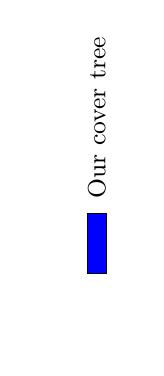
\begin{tikzpicture}
    \node[draw,fill=blue,minimum width=0.05in,minimum height=0.3in] at (0.3in,0) {};
    \node at (0.3in,0.63in) {\small\rotatebox{90}{Our cover tree}};
    \node[minimum width=0.05in,minimum height=0.3in] at (0.45in,0) {};
    \node at (0.45in,0.61in) {\small\rotatebox{90}{}};
    \node at (0,-0.475in) {};
\end{tikzpicture}
\end{center}

\vspace{0.1in}
Experiments run on an Amazon AWS instance with 16 true cores
\end{frame}

%%%%%%%%%%%%%%%%%%%%%%%%%%%%%%%%%%%%%%%%%%%%%%%%%%%%%%%%%%%%%%%%%%%%%%%%%%%%%%%%

\begin{frame}[fragile]{Parallel tree construction really matters on larger data sets}


%on small datasets with cheap metrics, parallel construction is less useful

\vspace{0.1in}
On large datasets with an expensive metric, parallelism is more useful

\vspace{0.15in}
Yahoo! Flickr dataset with 1.5 million images and earth mover distance

%\vspace{0.2in}
\vspace{0.15in}
\begin{center}
\Large
\begin{tabular}{ccccc}
\hline
num cores
 & \multicolumn{2}{c}{simplified tree} & \multicolumn{2}{c}{nearest ancestor tree} \\
%& \multicolumn{2}{c}{construction} & \multicolumn{2}{c}{construction} \\ %\cline{2-5}
& time & speedup & time & speedup \\
\hline
\hline
1  & 70.7 min & 1.0 & 210.9 min& 1.0\\
2  & 36.6 min & 1.9 & 94.2 min & 2.2\\
4  & 18.5 min & 3.8 & 48.5 min & 4.3\\
8  & 10.2 min & 6.9 & 25.3 min & 8.3\\
16 & 6.7 min & 10.5 & 12.0 min & 17.6\\
\hline
\end{tabular}
\end{center}

\end{frame}

%%%%%%%%%%%%%%%%%%%%%%%%%%%%%%%%%%%%%%%%%%%%%%%%%%%%%%%%%%%%%%%%%%%%%%%%%%%%%%%%

\begin{frame}[fragile]{The effect of parallel tree \emph{construction and query}}
\begin{center}
\graphicspath{{slides/paperimg/}}
% GNUPLOT: LaTeX picture with Postscript
\begingroup
  \makeatletter
  \providecommand\color[2][]{%
    \GenericError{(gnuplot) \space\space\space\@spaces}{%
      Package color not loaded in conjunction with
      terminal option `colourtext'%
    }{See the gnuplot documentation for explanation.%
    }{Either use 'blacktext' in gnuplot or load the package
      color.sty in LaTeX.}%
    \renewcommand\color[2][]{}%
  }%
  \providecommand\includegraphics[2][]{%
    \GenericError{(gnuplot) \space\space\space\@spaces}{%
      Package graphicx or graphics not loaded%
    }{See the gnuplot documentation for explanation.%
    }{The gnuplot epslatex terminal needs graphicx.sty or graphics.sty.}%
    \renewcommand\includegraphics[2][]{}%
  }%
  \providecommand\rotatebox[2]{#2}%
  \@ifundefined{ifGPcolor}{%
    \newif\ifGPcolor
    \GPcolortrue
  }{}%
  \@ifundefined{ifGPblacktext}{%
    \newif\ifGPblacktext
    \GPblacktextfalse
  }{}%
  % define a \g@addto@macro without @ in the name:
  \let\gplgaddtomacro\g@addto@macro
  % define empty templates for all commands taking text:
  \gdef\gplbacktext{}%
  \gdef\gplfronttext{}%
  \makeatother
  \ifGPblacktext
    % no textcolor at all
    \def\colorrgb#1{}%
    \def\colorgray#1{}%
  \else
    % gray or color?
    \ifGPcolor
      \def\colorrgb#1{\color[rgb]{#1}}%
      \def\colorgray#1{\color[gray]{#1}}%
      \expandafter\def\csname LTw\endcsname{\color{white}}%
      \expandafter\def\csname LTb\endcsname{\color{black}}%
      \expandafter\def\csname LTa\endcsname{\color{black}}%
      \expandafter\def\csname LT0\endcsname{\color[rgb]{1,0,0}}%
      \expandafter\def\csname LT1\endcsname{\color[rgb]{0,1,0}}%
      \expandafter\def\csname LT2\endcsname{\color[rgb]{0,0,1}}%
      \expandafter\def\csname LT3\endcsname{\color[rgb]{1,0,1}}%
      \expandafter\def\csname LT4\endcsname{\color[rgb]{0,1,1}}%
      \expandafter\def\csname LT5\endcsname{\color[rgb]{1,1,0}}%
      \expandafter\def\csname LT6\endcsname{\color[rgb]{0,0,0}}%
      \expandafter\def\csname LT7\endcsname{\color[rgb]{1,0.3,0}}%
      \expandafter\def\csname LT8\endcsname{\color[rgb]{0.5,0.5,0.5}}%
    \else
      % gray
      \def\colorrgb#1{\color{black}}%
      \def\colorgray#1{\color[gray]{#1}}%
      \expandafter\def\csname LTw\endcsname{\color{white}}%
      \expandafter\def\csname LTb\endcsname{\color{black}}%
      \expandafter\def\csname LTa\endcsname{\color{black}}%
      \expandafter\def\csname LT0\endcsname{\color{black}}%
      \expandafter\def\csname LT1\endcsname{\color{black}}%
      \expandafter\def\csname LT2\endcsname{\color{black}}%
      \expandafter\def\csname LT3\endcsname{\color{black}}%
      \expandafter\def\csname LT4\endcsname{\color{black}}%
      \expandafter\def\csname LT5\endcsname{\color{black}}%
      \expandafter\def\csname LT6\endcsname{\color{black}}%
      \expandafter\def\csname LT7\endcsname{\color{black}}%
      \expandafter\def\csname LT8\endcsname{\color{black}}%
    \fi
  \fi
  \setlength{\unitlength}{0.0500bp}%
  \begin{picture}(5040.00,3772.00)%
    \gplgaddtomacro\gplbacktext{%
      \csname LTb\endcsname%
      \put(1254,1129){\makebox(0,0)[r]{\strut{}$2^{-4}$}}%
      \csname LTb\endcsname%
      \put(1254,1526){\makebox(0,0)[r]{\strut{}$2^{-3}$}}%
      \csname LTb\endcsname%
      \put(1254,1922){\makebox(0,0)[r]{\strut{}$2^{-2}$}}%
      \csname LTb\endcsname%
      \put(1254,2318){\makebox(0,0)[r]{\strut{}$2^{-1}$}}%
      \csname LTb\endcsname%
      \put(1254,2714){\makebox(0,0)[r]{\strut{}$2^{+0}$}}%
      \csname LTb\endcsname%
      \put(1254,3111){\makebox(0,0)[r]{\strut{}$2^{+1}$}}%
      \put(1873,601){\rotatebox{-45}{\makebox(0,0)[l]{\strut{}yearpredict}}}%
      \put(1873,381){\rotatebox{-45}{\makebox(0,0)[l]{\strut{}(277min)}}}%
      \put(2471,601){\rotatebox{-45}{\makebox(0,0)[l]{\strut{}twitter}}}%
      \put(2471,381){\rotatebox{-45}{\makebox(0,0)[l]{\strut{}(51min)}}}%
      \put(3068,601){\rotatebox{-45}{\makebox(0,0)[l]{\strut{}tinyImages}}}%
      \put(3068,381){\rotatebox{-45}{\makebox(0,0)[l]{\strut{}(34min)}}}%
      \put(3666,601){\rotatebox{-45}{\makebox(0,0)[l]{\strut{}mnist}}}%
      \put(3666,381){\rotatebox{-45}{\makebox(0,0)[l]{\strut{}(30min)}}}%
      \put(176,2120){\rotatebox{-270}{\makebox(0,0){\strut{}normalized total runtime}}}%
      \put(396,2120){\rotatebox{-270}{\makebox(0,0){\strut{}(both \emph{construction} and \emph{query})}}}%
      \put(616,2120){\rotatebox{-270}{\makebox(0,0){\strut{}  }}}%
      \put(1774,2980){\makebox(0,0)[l]{\strut{}\tiny 1}}%
      \put(1849,3174){\makebox(0,0)[l]{\strut{}\tiny 1}}%
      \put(1924,2814){\makebox(0,0)[l]{\strut{}\tiny 1}}%
      \put(1983,2453){\makebox(0,0)[l]{\strut{}\tiny 2}}%
      \put(2058,1954){\makebox(0,0)[l]{\strut{}\tiny 4}}%
      \put(2124,1648){\makebox(0,0)[l]{\strut{}\tiny 8}}%
      \put(2184,1399){\makebox(0,0)[l]{\strut{}\tiny 16}}%
    }%
    \gplgaddtomacro\gplfronttext{%
    }%
    \gplbacktext
    \put(0,0){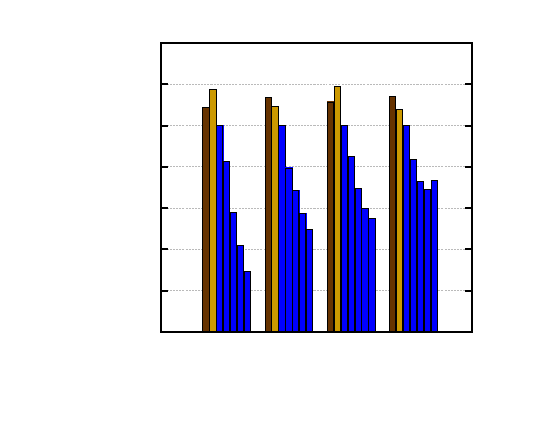
\includegraphics{parallel}}%
    \gplfronttext
  \end{picture}%
\endgroup

\definecolor{colorOrig}{RGB}{102,51,0}
\definecolor{colorMlpack}{RGB}{204,153,0}
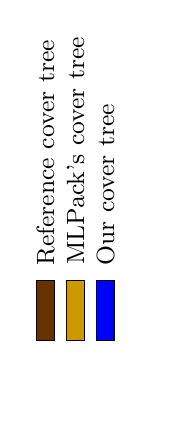
\begin{tikzpicture}
    \node[draw,fill=colorOrig,minimum width=0.05in,minimum height=0.3in] at (0,0) {};
    \node at (0,0.79in) {\small\rotatebox{90}{Reference cover tree}};
    \node[draw,fill=colorMlpack,minimum width=0.05in,minimum height=0.3in] at (0.15in,0) {};
    \node at (0.15in,0.80in) {\small\rotatebox{90}{MLPack's cover tree}};
    \node[draw,fill=blue,minimum width=0.05in,minimum height=0.3in] at (0.3in,0) {};
    \node at (0.3in,0.63in) {\small\rotatebox{90}{Our cover tree}};
    \node[minimum width=0.05in,minimum height=0.3in] at (0.45in,0) {};
    \node at (0.45in,0.61in) {\small\rotatebox{90}{}};
    \node at (0,-0.475in) {};
\end{tikzpicture}
\end{center}

\vspace{0.1in}
Experiments run on an Amazon AWS instance with 16 true cores
\end{frame}
